% File: 02-main/ch3_design.tex (Content for Results and Current Status)

\chapter{Results and Current Status}
\label{chap:results}

%\minitoc

This chapter presents current results of the MREyeQC project, focusing on the successful adaptation of the Image Quality Metric (IQM) computational pipeline, and the first results of learning-based quality prediction models.

\section{IQM Computation Pipeline for Ocular MRI: Validation and Output}
\label{sec:iqm_pipeline_validation}
By investigating relevant IQMs in the FetMRQCR project, the pipeline for computing all IQMs for ocular MRI is now operational. At the end of this pipeline, a CSV file is obtained that aggregates the results of each IQM for each subject tested. This dataset constitutes the direct input to the machine learning workflow for automated quality assessment.

\section{Correlation index of each IQM}
Analyzing the calculated IQM file manually proves to be complicated. Therefore, the correlation index of each IQM according to the desired result was calculated to observe which IQMs are most relevant for classifying the images. The result obtained is presented below.

\begin{table}[htbp]
    \centering
    \caption{Top 20 IQMs Correlated with 'Rating' (Absolute Values)}
    \label{tab:top_iqm_correlations}
    \begin{tabular}{lr}
        \toprule
        \textbf{IQM} & \textbf{Correlation Coefficient} \\
        \midrule
        seg\_snr\_GLOBE                   & 0.682922 \\
        seg\_cjv                        & -0.626543 \\
        seg\_sstats\_GLOBE\_mad           & -0.573834 \\
        seg\_sstats\_GLOBE\_stdv          & -0.550379 \\
        seg\_sstats\_GLOBE\_k              & 0.485470 \\
        seg\_snr\_total                   & 0.469745 \\
        seg\_cnr                         & 0.468125 \\
        seg\_sstats\_GLOBE\_p95           & -0.445921 \\
        centroid\_full                   & 0.359771 \\
        seg\_sstats\_MUSCLE\_k             & 0.355294 \\
        seg\_sstats\_OPTIQUE\_NERVE\_n      & 0.282753 \\
        mi\_median                      & -0.262807 \\
        seg\_sstats\_FAT\_mad             & -0.259243 \\
        shannon\_entropy                & -0.258915 \\
        mi\_window                      & -0.253138 \\
        seg\_sstats\_GLOBE\_p05            & 0.240962 \\
        seg\_lens\_aspect\_ratio          & -0.236386 \\
        seg\_sstats\_FAT\_stdv            & -0.236090 \\
        seg\_sstats\_OPTIQUE\_NERVE\_p95   & -0.232774 \\
        nmi\_median                     & -0.225741 \\
        \bottomrule
    \end{tabular}
\end{table}

\subsection{Observation}
First, it is observed that none of the IQMs achieved a very high correlation coefficient, with the maximum absolute correlation being 0.683 for seg\_snr\_GLOBE. This indicates that while useful, no single IQM perfectly aligns with human quality ratings in this dataset.

Notably, IQMs derived from the globe segmentation (GLOBE class) consistently show strong correlations with the ratings. In fact, among the top 8 correlated IQMs, all are based on segmentation features. This strongly suggests that the quality of anatomical segmentation is a crucial factor for accurately classifying image quality.

Conversely, it is important to highlight that none of the newly implemented IQMs appeared in the top 20 correlations. This suggests that initial hypotheses regarding these specific new metrics were not supported by the data, and they may not be effective indicators for image quality classification in this context.

\section{Machine Learning for Automated Quality Prediction: Initial Model Performance}
\label{sec:ml_results_revised}

The machine learning phase aimed to develop a model capable of predicting image quality from the calculated image quality indicators (IQMs). This section details the characteristics of the dataset, the model training method, and preliminary performance results.
As illustrated in Figure~\ref{fig:combined_rating_distributions}, the distribution of the original multi-category ratings (Exclude, Poor, Acceptable, Excellent) highlights a non-homogeneous representation across classes. For the purpose of binary classification, these ratings were consolidated into "reject" (corresponding to the "excluded" category) and "accept" (encompassing "poor," "acceptable," and "excellent"). The resulting binary distribution, shown in Figure~\ref{fig:combined_rating_distributions}, underscores a class imbalance, which necessitated specific considerations during model training. The relatively small total dataset size (N=83) inherently presents challenges for model generalization and amplifies the sensitivity of performance metrics to data splits.

\begin{figure}[htbp]
    \centering
    \begin{subfigure}[b]{0.48\textwidth}
        \centering
        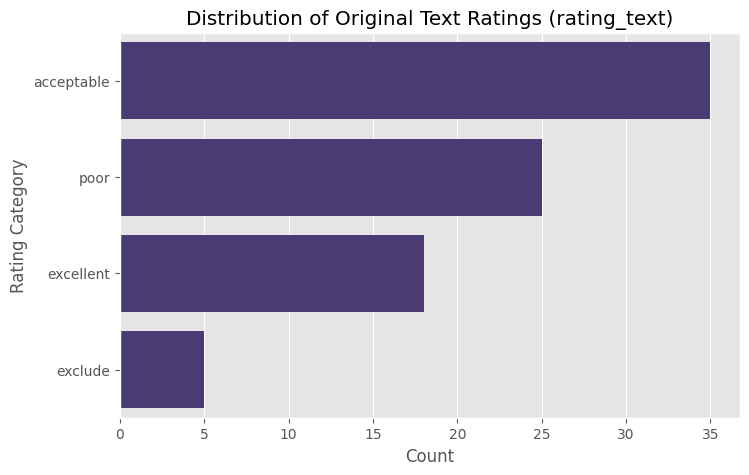
\includegraphics[width=\linewidth]{Report/img/Distrubution_of_rating.png}
        \label{subfig:rating_distribution_detailed}
    \end{subfigure}
    \hfill
    \begin{subfigure}[b]{0.48\textwidth} % Second subfigure, 48% of text width
        \centering
        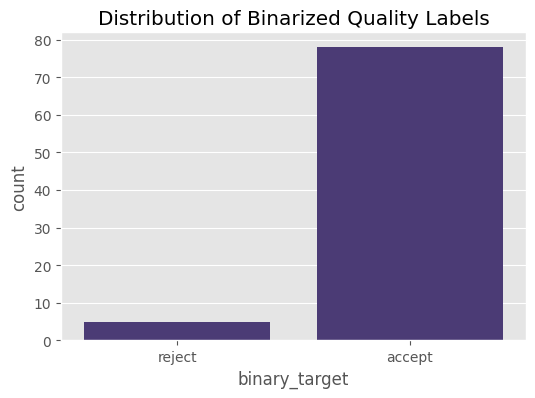
\includegraphics[width=\linewidth]{Report/img/Distrubution_of_quality.png}
        \label{subfig:quality_distribution_binary}
    \end{subfigure}
    \caption{Comparison of manual image quality rating distributions: (a) Original multi-category ratings (Exclude, Poor, Acceptable, Excellent) across 83 images, and (b) Binarized quality labels ("reject" vs. "accept") used for model training.}
    \label{fig:combined_rating_distributions}
\end{figure}

A Random Forest classifier was chosen as the training model. The dataset was subsequently partitioned into training (75\%) and testing (25\%) sets using stratified sampling to maintain class proportions across both splits. Standard preprocessing involved feature scaling via StandardScaler. To address class imbalance, the Random Forest model was configured with class\_weight='balanced'. Hyperparameter tuning was performed using 5-fold stratified cross-validation on the training set, with ROC AUC as the optimization metric. The final model's optimized parameters were: n\_estimators=100, max\_depth=20, min\_samples\_split=5, and min\_samples\_leaf=2.

\subsection{Prediction Generation and Preliminary Model Efficacy}
\label{ssec:model_efficacy_revised} 

The optimized Random Forest classifier was subsequently utilized to generate automated quality predictions on the held-out test set. This test set comprised 20 images, consisting of 3 'reject' cases (15.0\% of the test set) and 17 'accept' cases (85.0\% of the test set)

\begin{table}[htbp]
\centering
\caption{Per-Class Performance Metrics on the Test Set for the Random Forest Model}
\label{tab:per_class_metrics_revised}
\begin{tabular}{lccc}
\toprule
\textbf{Class} & \textbf{Precision} & \textbf{Recall (Sensitivity)} & \textbf{F1-score} \\
\midrule
Reject (Class 0) & \textit{0.00} & \textit{0.00} & \textit{1} \\
Accept (Class 1) & \textit{0.95} & \textit{1.0} & \textit{0.98} \\
\bottomrule
\end{tabular}
\end{table}

The confusion matrix for the test set and The Receiver Operating Characteristic (ROC) curve are presented in Figure~\ref{fig:model_performance}.
\begin{figure}[htbp]
    \centering
    \begin{subfigure}[b]{0.48\textwidth}
        \centering
        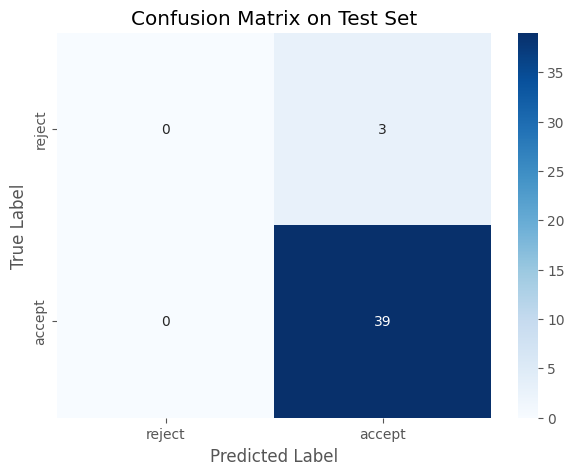
\includegraphics[width=\linewidth]{Report/img/confusion_matrix_model.png} 
        \label{subfig:confusion_matrix} 
    \end{subfigure}
    \hfill
    \begin{subfigure}[b]{0.48\textwidth} 
        \centering
        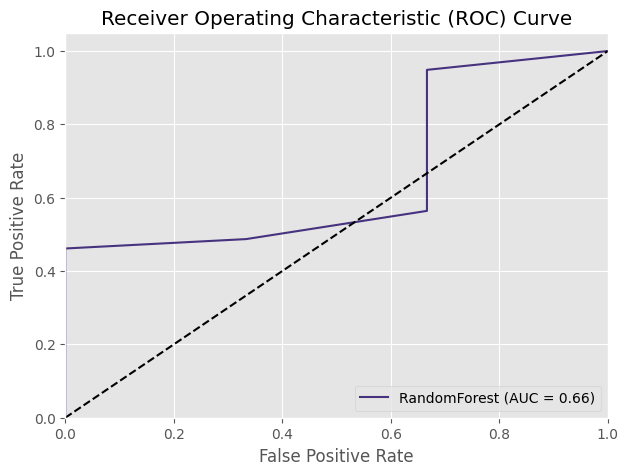
\includegraphics[width=\linewidth]{Report/img/ROC_Curve.png} % Your path
        % No individual caption for subfigure
        \label{subfig:roc_curve} % Unique label for this subfigure
    \end{subfigure}
    \caption{Performance of the Random Forest model on the test set: (a) Confusion matrix, illustrating true/false positives and negatives for the "accept" and "reject" classes; and (b) Receiver Operating Characteristic (ROC) curve with an Area Under the Curve (AUC) of $0.6581$.}
    \label{fig:model_performance} 
\end{figure}
\newpage
\begin{figure}[H]
    \centering
    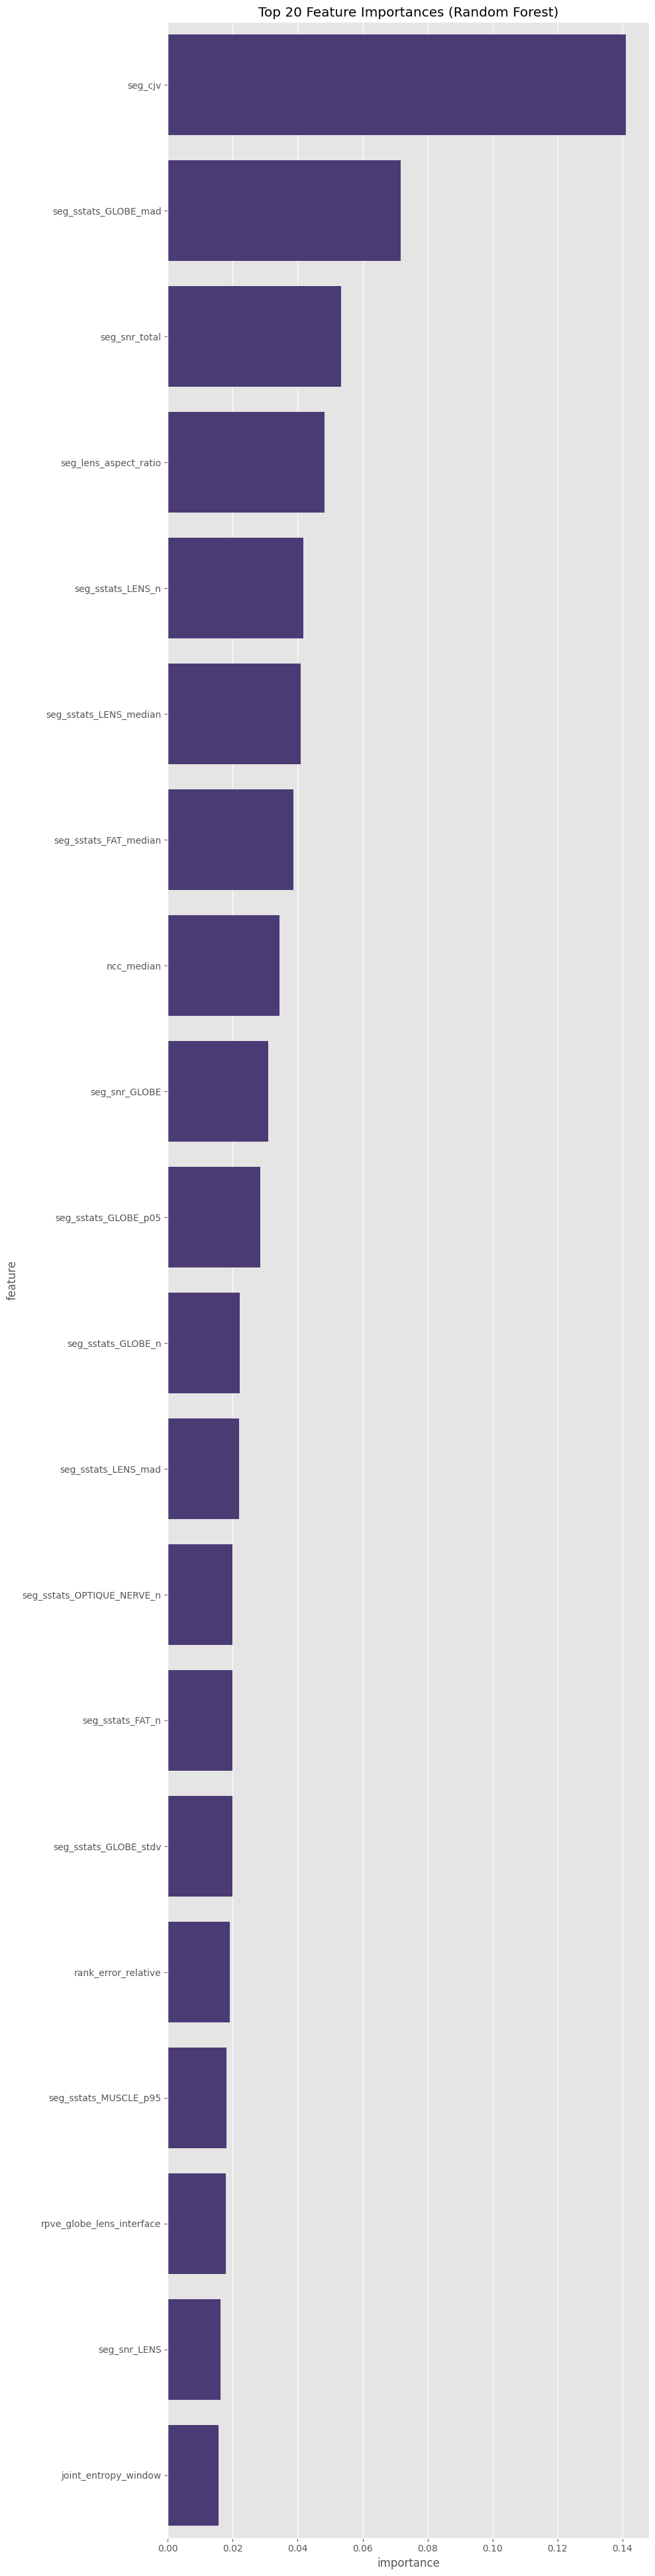
\includegraphics[width=0.4\textwidth]{Report/img/Feature_random_forest.png}
    \caption{Top N feature importances from the Random Forest model, indicating the relative contribution of different IQMs to the quality prediction.}
    \label{fig:feature_importances_results} 
\end{figure}
\newpage
\noindent \textbf{Interpretation of Preliminary Results:}
The reported overall accuracy of $0.9286$ appears high. However, the ROC AUC of $0.6581$ suggests a modest discriminative ability of the model across all decision thresholds. Given the imbalanced nature of the test set, the high overall accuracy and the reported recall of $1.0$ and F1-score of $0.9630$ are likely dominated by the model's performance on the majority "accept" class. 

The critical evaluation hinges on the Balanced Accuracy and the recall for the "reject" class. A Balanced Accuracy significantly lower than the overall accuracy would confirm the influence of class imbalance. For instance, if the recall for the "reject" class is low, it would mean that while most good quality images are correctly classified, a substantial portion of poor quality ("excluded") images are being missed (false negatives for the "reject" class). Conversely, the precision for the "reject" class would indicate the rate of false alarms.

These initial findings, while demonstrating the feasibility of training a predictive model, highlight the challenges posed by the small dataset size and class imbalance. The current ROC AUC suggests room for improvement in the model's overall ability to separate the classes robustly. Future work will focus on.